\documentclass{beamer}
\beamertemplatenavigationsymbolsempty
\usecolortheme{beaver}
\setbeamertemplate{blocks}[rounded=true, shadow=true]
\setbeamertemplate{footline}[page number]
%
\usepackage[utf8]{inputenc}
\usepackage[english,russian]{babel}
\usepackage{amssymb,amsfonts,amsmath,mathtext}
\usepackage[]{algorithmic}
\usepackage{subfig}
\usepackage[all]{xy} % xy package for diagrams
\usepackage{array}
\usepackage{tikz}
\usepackage{multicol}% many columns in slide
\usepackage{hyperref}% urls
\usepackage{hhline}%tables
\usepackage{biblatex}
% Your figures are here:
\graphicspath{ {fig/} {../fig/} }
\usepackage{graphicx}
\usepackage{subcaption}
\usepackage{wrapfig}
\usepackage{amsmath}
\usepackage{caption}
\captionsetup{labelformat=empty}
\usepackage{subfigure}
\newcommand\normx[1]{\left\Vert#1\right\Vert}

\newcommand\myfootnote[1]{%
  \tikz[remember picture,overlay]
  \draw (current page.south west) +(1in + \oddsidemargin,0.5em)
  node[anchor=south west,inner sep=0pt]{\parbox{\textwidth}{%
      \rlap{\rule{10em}{0.4pt}}\raggedright\scriptsize \textit{#1}}};}

%----------------------------------------------------------------------------------------------------------
\title[\hbox to 56mm{Векторное представление моделей}]{Методы векторного представления глубоких генеративных моделей}
\author[М.\,А. Никитина]{Мария Александровна Никитина}
\institute{Московский физико-технический институт}
\date{\footnotesize
\par\smallskip\emph{Кафедра:} Интеллектуальный анализ данных
\par\smallskip\emph{Научный руководитель:} кандидат ф.-м. наук О.\,Ю.~Бахтеев
\par\smallskip\emph{Научный консультант:} А.\,Ю.~Бишук
\par\bigskip\small 2025}
%----------------------------------------------------------------------------------------------------------
\begin{document}
%----------------------------------------------------------------------------------------------------------
\begin{frame}
\thispagestyle{empty}
\maketitle
\end{frame}
%-----------------------------------------------------------------------------------------------------
\begin{frame}{Задача векторного описания генеративных моделей}
% \footnotesize
\begin{block}{Задача}
Задан набор генеративных моделей, описывающий разные выборки/генеральные совокупности данных. Требуется предложить метод векторного представления этих моделей, который будет представлять их статистические свойства.
\end{block}
\begin{block}{Требования}
\begin{enumerate}
    \item Расстояние между векторными представлениями моделей для близких выборок должно быть невелико (при условии, что сами модели хорошо их описывают)
    \item Модели, обученные на композиции/смеси выборок должны учитывать свойства всех выборок, входящих в смесь
\end{enumerate}
\end{block}
\end{frame}
%-----------------------------------------------------------------------------------------------------
\begin{frame}{Свойства пространства}
\begin{wrapfigure}{r}{0.35\textwidth}
  \vspace{-20pt}
  \begin{center}
    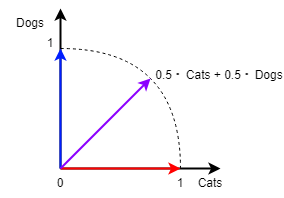
\includegraphics[width=0.4\textwidth]{Pictures/Classes.png}
  \end{center}
  \vspace{-20pt}
\end{wrapfigure}
1. Сумма векторных представлений моделей, полученных по датасетам $D_1$, $D_2$ должна приблизительно соответствовать векторному представлению датасета $D_1 + D_2$;

\bigskip

2. Вместо евклидового расстояния на векторных представлениях, используется иерархия;
\end{frame}
%----------------------------------------------------------------------------------------------------------
\begin{frame}{Бинарная классификация по датасету обучения}
\begin{block}{Мотивация}
Если нужно создать вектор модели с требуемым свойством, то сначала следует проверить, насколько хорошо вектор модели описывает данные, используемые для обучения.
\end{block}
\begin{block}{Метод}
Обучение бинарного классификатора на определение датасета, из которого была взята выборка для обучения автоэнкодера.
\end{block}
\begin{block}{Вход классификатора}
Чтобы не допустить переобучения классификатора и не завязываться на размерности, энкодеры векторизуются:

\begin{enumerate}
    \item Сингулярные числа весов
    \item Гистограмма значений весов
\end{enumerate}
\end{block}
\end{frame}
%----------------------------------------------------------------------------------------------------------
\begin{frame}{Теоретические оценки на потерю информации}
\small
\begin{block}{Теорема (Никитина, 2025)}
$X = \{\mathbf{x}_1, \dots, \mathbf{x}_n\} \in \mathbb{R}^{n \times d}$ -- множество независимых векторов (пусть $\mathbf{x}_i \in \mathbb{R}^d$ и $\mathbf{x}_i \sim \mathcal{N}(\boldsymbol{\mu}, \boldsymbol{\Sigma})$).

$X_1 \in \mathbb{R}^{m \times d}$ -- его подмножество, формируемое путём независимого включения каждого вектора $\mathbf{x}_i$ с вероятностью $p$.

$AE$ -- линейный автоэнкодер с весами $W \in \mathbb{R}^{k\times d}$. $AE$ обучен на $X_1$, то есть $W = W(X_1)$. $\mathbf{s}$ -- вектор сингулярных чисел $AE$.

Тогда имеем следующие попарные взаимные информации:

\begin{enumerate}
    \item \[I(X; X_1) \approx np \cdot H(\mathbf{x}_i), ~~~  H(\mathbf{x}_i) = \frac{1}{2} \log \left( (2 \pi e)^d |\Sigma| \right);\]

    \item \[I(X_1; W) = \frac{m}{2} \log \frac{|\boldsymbol{\Sigma}|}{|(\mathbf{I} - \mathbf{W}_2 \mathbf{W}_1) \boldsymbol{\Sigma} (\mathbf{I} - \mathbf{W}_2 \mathbf{W}_1)^T|}\]

    \item \[I(X_1; \mathbf{s}) \approx \frac{m}{4} \log \left( (2\pi e)^k \prod_{i=1}^k \lambda_i^2 \right).\]
\end{enumerate}
\end{block}
\end{frame}
%----------------------------------------------------------------------------------------------------------
\begin{frame}{Схема базовой задачи}
\begin{figure}
    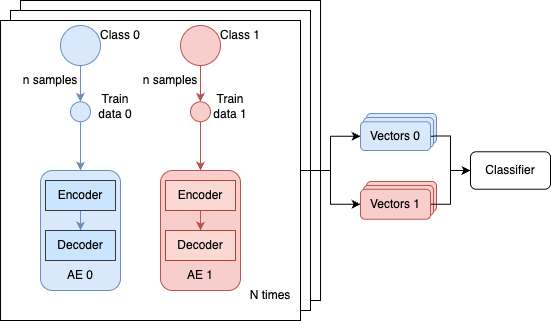
\includegraphics[width=1.0\linewidth]{Presentation/Pictures/vector_space.png}
    \caption{От классификатора требуется предсказывать класс, на котором обучен автоэнкодер.}
\end{figure}
\end{frame}
%----------------------------------------------------------------------------------------------------------
\begin{frame}{Метрики базовой задачи}
\begin{table}[!ht]
\begin{center}
\caption{Метрики качества предсказания класса, на котором обучалась модель}
\begin{tabular}{| c | c | c |}
\hline
& Precision & Recall \\ \hline
1 линейный слой & 0.79 & 1.00 \\ \hline
1 свёрточный слой & 0.55 & 0.78 \\ \hline
\end{tabular}
\end{center}
\end{table}

Автоэнкодеры с линейным слоем, обученные на разных датасетах, отличить друг от друга легче, чем автоэнкодеры со свёрточными слоями. То есть, чем сложнее модель, тем больше информации теряется о ней и датасете при обучении и векторизации.
\end{frame}
%----------------------------------------------------------------------------------------------------------
\begin{frame}{Построение векторного пространства}
Берётся 3 наиболее удалённых класса из датасета CIFAR. Для поиска таких классов используется евклидово расстояние на ембеддингах, полученных из выходного слоя ResNet.

\begin{block}{Алгоритм}
\begin{enumerate}
    \item Случайное сэмплирование долей классов в датасете для $N$ моделей;

    \item Обучение $N$ моделей на соответствующих датасетах;

    \item Получение векторов из обученных моделей;

    \item Обучение энкодера на полученных моделях. Предсказание:
        \begin{enumerate}
            \item Вектора на части единичной сферы

            \item Расстояния между двумя моделями
        \end{enumerate}
\end{enumerate}
\end{block}
\end{frame}
%----------------------------------------------------------------------------------------------------------
\begin{frame}{Схема эксперимента}
\begin{figure}
    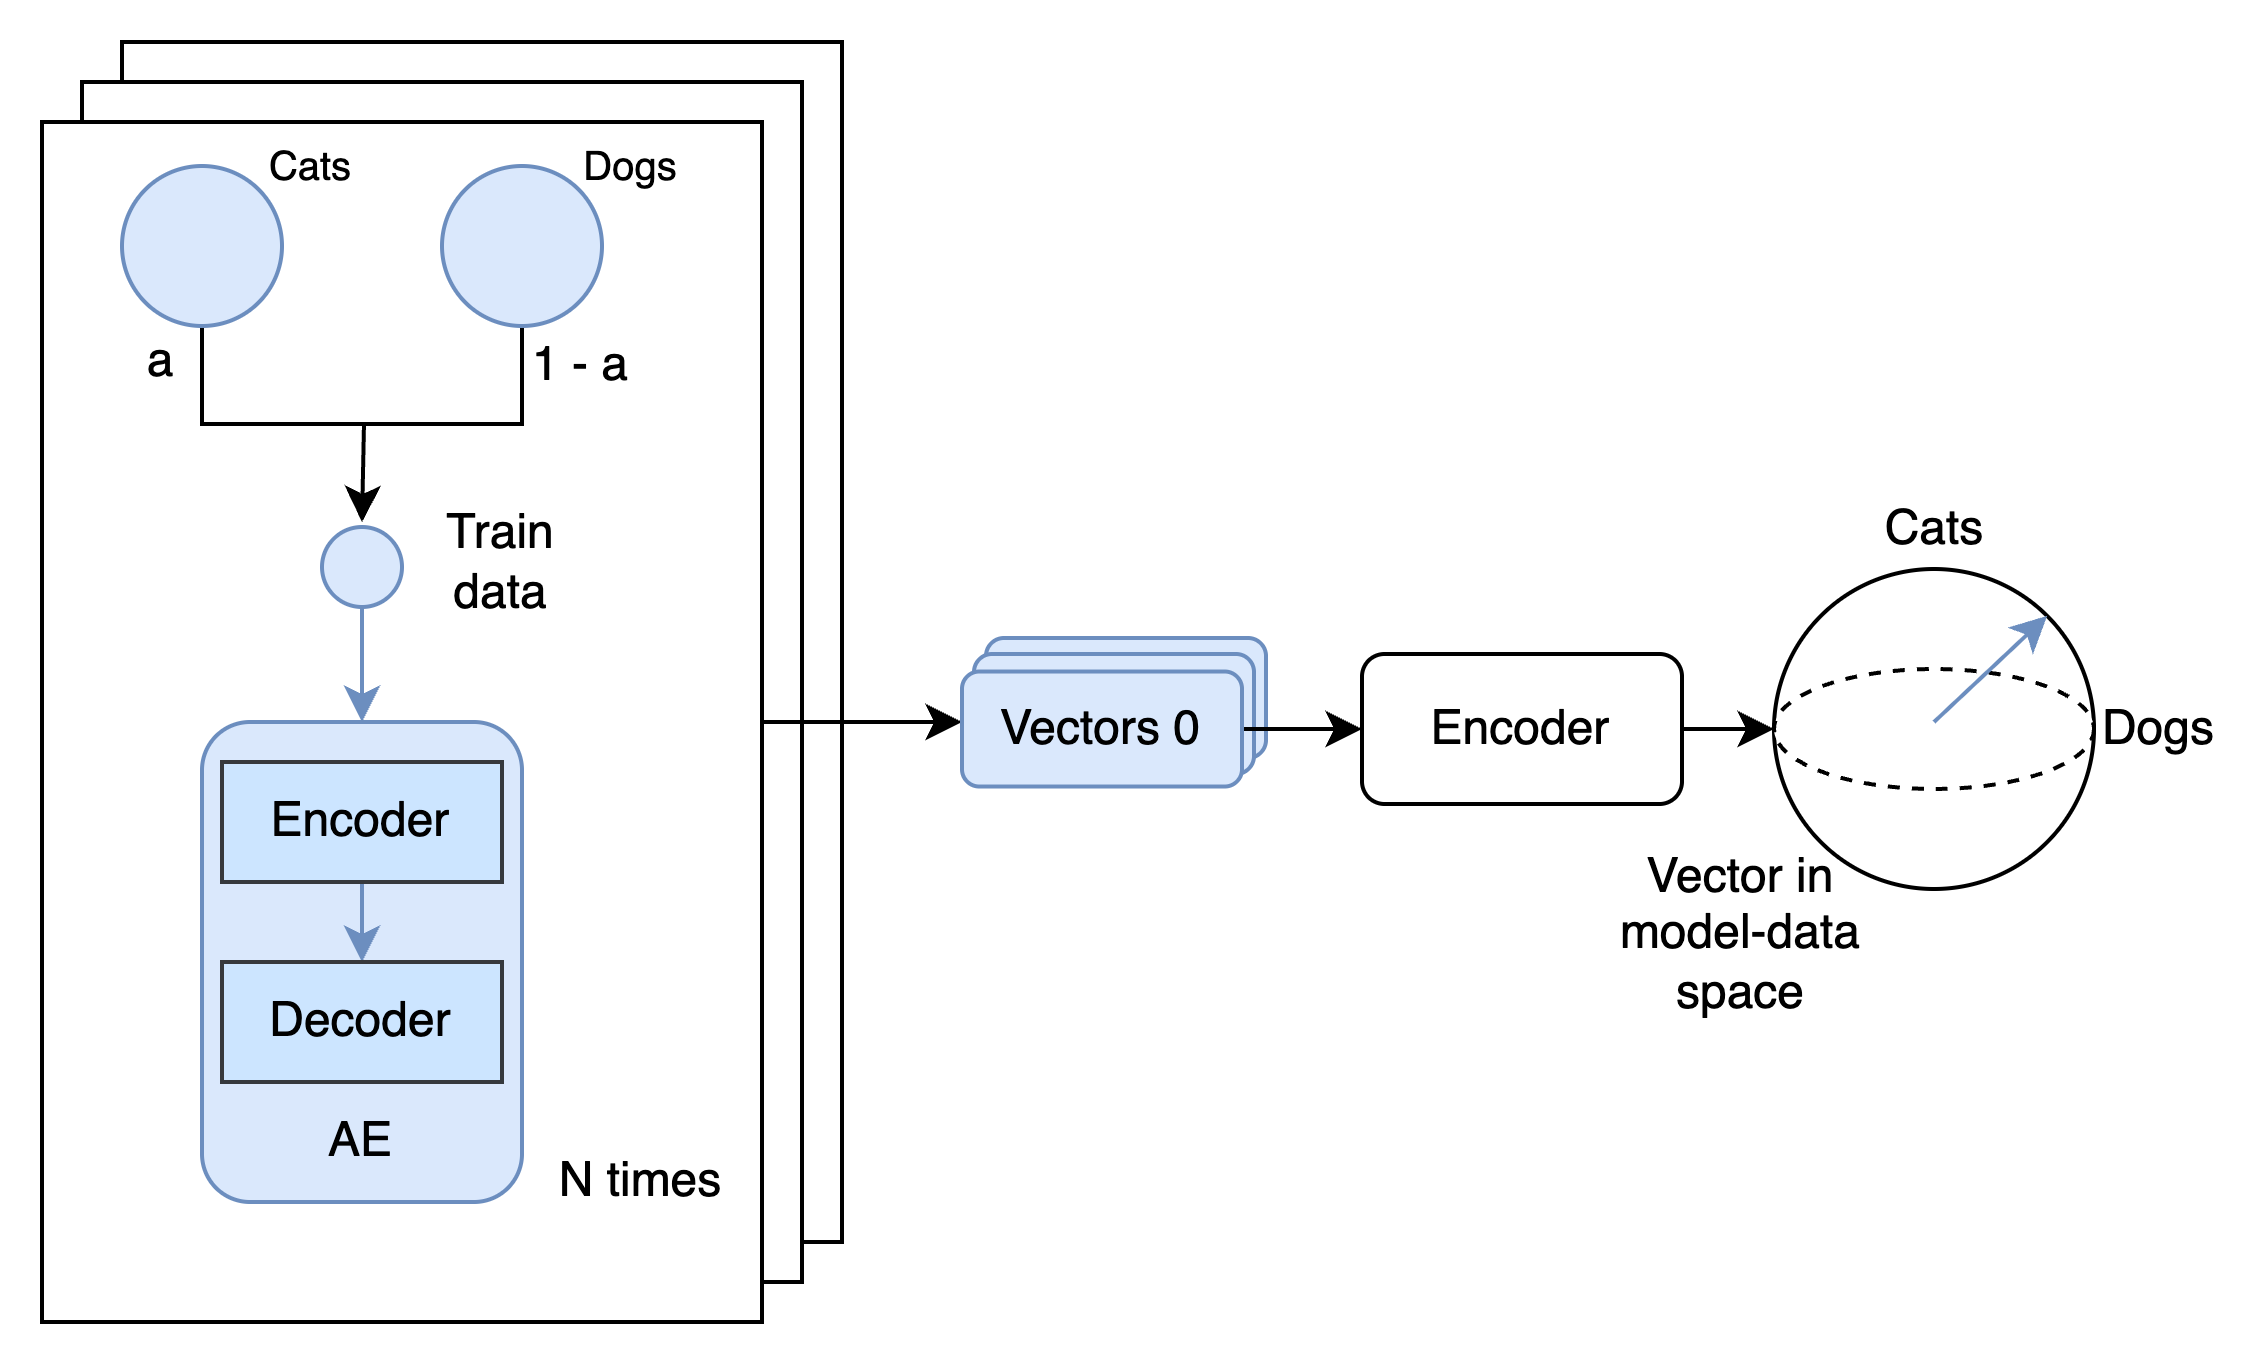
\includegraphics[width=1.0\linewidth]{Pictures/experiment.png}
    \caption{Задача энкодера: приблизить вектор обученной модели к вектору датасета}
\end{figure}
\end{frame}
%----------------------------------------------------------------------------------------------------------
\begin{frame}{Среднее векторов скрытого пространства}

\begin{wrapfigure}{r}{0.45\textwidth}
  \vspace{-30pt}
  \begin{center}
    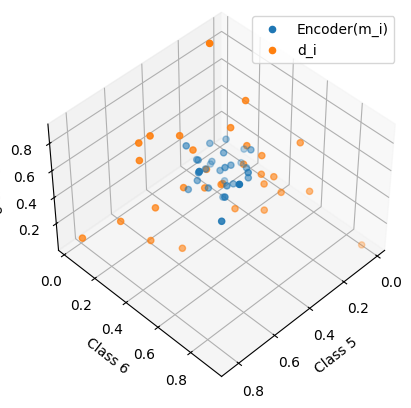
\includegraphics[width=0.5\textwidth]{Pictures/Encoder.png}
  \end{center}
  \vspace{-20pt}
\end{wrapfigure}

\textit{Способ представления модели}: среднее значение скрытого пространства автоэнкодера на тестовой выборке.

\bigskip

\textit{Функция потерь энкодера}: MSE

\bigskip

\textit{Проблемы}: Переобучение энкодера и неинформативность взятия среднего
\end{frame}
%----------------------------------------------------------------------------------------------------------
\begin{frame}{Сингулярные числа весов модели}

\begin{wrapfigure}{r}{0.45\textwidth}
  \vspace{-30pt}
  \begin{center}
    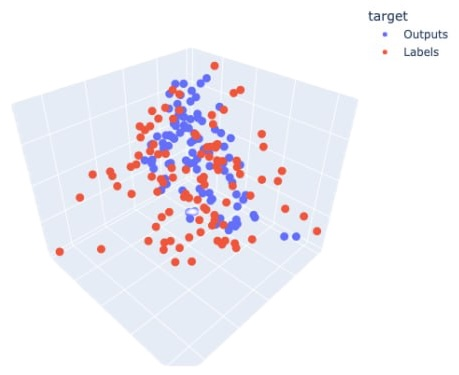
\includegraphics[width=0.5\textwidth]{Pictures/singular.jpg}
  \end{center}
  \vspace{-20pt}
\end{wrapfigure}

\textit{Способ представления модели}: Для матриц весов автоэнкодера считаются сингулярные числа. Затем все значения вытягиваются в один вектор.

\bigskip

\textit{Функция потерь энкодера}: MSE

\bigskip

\textit{Проблемы}: При увеличении числа слоёв увеличивается число сингулярных чисел, а, значит, метод не масштабируется на различные архитектуры.
\end{frame}
%----------------------------------------------------------------------------------------------------------
\begin{frame}{Выводы}
\begin{enumerate}
    \item Продолжить предложенные эксперименты: результаты первого показывают, что подход требует аккуратного анализа и изменения деталей эксперимента. Например, строить вектор модели не по результату её работы на случайных сэмплах, а по её весам.

    \item Поставить эксперименты с VAE-моделью. Трудности: тяжело подобрать веса так, чтобы картинка получилась не размытой.

    \item Описать результаты экспериментов с теоретической точки зрения.
\end{enumerate}
\end{frame}
%----------------------------------------------------------------------------------------------------------
% \begin{frame}{Список литературы}
% \begin{thebibliography}{99} 
%     \footnotesize
    
%     \bibitem[Chuang, 2020]{p1}
%         Ching-Yao Chuang, Joshua Robinson, Lin Yen-Chen, Antonio Torralba, Stefanie Jegelkah (2020)
%         \newblock Debiased Contrastive Learning

%         \bibitem[Yang, 2022]{p2}
%         Yang, Jinyu and Duan, Jiali and Tran, Son and Xu, Yi and Chanda, Sampath and Chen, Liqun and Zeng, Belinda and Chilimbi, Trishul and Huang, Junzhou (2022)
%         \newblock Vision-Language Pre-Training with Triple Contrastive Learning

%        \bibitem[Chen2020SimCLR, 2020]{p3}
%         CTing Chen, Simon Kornblith, Mohammad Norouzi, Geoffrey Hinton (2020)
%         \newblock A Simple Framework for Contrastive Learning of Visual Representations

%     \bibitem[VQA, 2017]{p4}
%         Stanislaw Antol and Aishwarya Agrawal and Jiasen Lu and Margaret Mitchell and Dhruv Batra and C. Lawrence Zitnick and Devi Parikh (2017)
%         \newblock {VQA}: {V}isual {Q}uestion {A}nswering

%     \bibitem[schroff2015facenet, 2015]{p5}
%         Florian Schroff, Dmitry Kalenichenko, James Philbin (2015)
%         \newblock FaceNet: A Unified Embedding for Face Recognition and Clustering

% \end{thebibliography}
% \end{frame}
\end{document} 
